\documentclass[12pt]{article}
\usepackage{fontspec}
\usepackage{titling}
\usepackage[portuguese]{babel}
\renewcommand{\baselinestretch}{1.5} 
\usepackage{csquotes}
\usepackage{graphicx}
\usepackage{adjustbox}
\usepackage{lipsum}
\usepackage[backend=biber,autolang=other,
  bibencoding=utf8,style=authoryear-ibid,
  ibidtracker=true]{biblatex}

\setmainfont[]{Times New Roman}

\usepackage[margin=2cm,left=3cm]{geometry}

\addbibresource{viagem.bib}

\title{Viagem à volta do meu quarto}
\date{10 de Dezembro de 2015}
\author{João Távora \\Faculdade de Belas Artes da Universidade de Lisboa}

\begin{document}
%% DONE: le tértre, o que é?
%% TODO: Bibliografia, maketitle
%% TODO: Muitas referências a acidentes
%% DONE: Imagem quadro do van gogh

\emph{Viagem à volta do meu quarto}\\
\emph{João Távora}\\
\emph{Faculdade de Belas Artes da Universidade de Lisboa}\\
\emph{10 de Dezembro de 2015}\\

\section{Resumo}

Estuda-se ``Viagem à volta do meu quarto'', pequeno livro de 1795 de
Xavier de Maistre, paródia da literatura de viagens popular na altura,
procurando nele pistas sobre os processos criativos ligados
principalmente à prática artística da Pintura e do Desenho, destapando
a sua influência noutras obras, desde a sua publicação até ao
presente, propondo paralelos entre o texto e alguns autores da
filosofia, da poesia e das artes plásticas.

\section{Introdução}

``Viagem à volta do meu quarto'' é o título que Xavier de Maistre deu
ao livro que escreveu em 1795 e no qual descreve o período de 42 dias
de prisão domiciliária que lhe é imposto por envolvimento num duelo. O
livro é um diário desse cárcere real, escrito em jeito de romance de
viagems, num percurso imaginado e acidentado pelas memórias que o
espaço desse quarto evoca no protagonista. Trata-se de uma paródia da
literatura deste género, particularmente estimada na época em que o
``Grand Tour'' europeu era um ritual iniciático na vida de qualquer
jovem aristocrático. A este livro, de Maistre somou outro em 1825,
chamado ``Expedição noctura à volta do meu quarto''. Ambos se
encontram estruturados em tantos capítulos quantos dias duraram as
respectivas viagens.

Param além de comédias, estes livros são uma defesa da imaginação e da
intimidade afectiva como fontes de descoberta intelectual e
criativa. Escritos durante a turbulência da revolução francesa, na
eclosão da modernidade, influenciaram escritores e artistas plásticos
até ao presente. O presente texto tem como objecto destapar alguns
aspectos particulares da obra de Maistre que possam constituir
incursões nos processos das artes plásticas, sobretudo na Pintura e no
Desenho.

\section{Desenvolvimento}

\subsection{Da paródia à inquietação filosófica}

Nas primeiras linhas de Maistre anuncia imodestamente que ``aparece de
repente no mundo erudito'' com um ``livro de descobertas na
mão''. Viajar no próprio quarto é ``um meio seguro contra o tédio'' e
a cómoda e democrática forma de viajar: serve os indolentes, os
indigentes, os medrosos.

O principal dispositivo lúdico é o simulacro de viagem, excutado com
insólita precisão. Descreve-se convincentemente um levantamento
topológico do espaço do quarto, viagens a cavalo do parapeito da
janela, reuniões, separações e imprevistos. Mas cada relato acaba por
expõr também a banalidade desse quarto e do carácter indolente e
ridículo do seu habitante vestido de \emph{roupão de viagem}, viajante
fechado no quarto.

A paródia consiste em que algum desse ridículo se transfere para o
referente e e troce também da grandiosidade dos relatos de viagens
reais. A disparadidade absurda da comparação faz ainda com que esse
comentário se transforme em inquietação filosófica. Nessa dimensão
quase sinistra - não faz diferença nenhuma se viajamos pelo nosso
quarto ou por qualquer lugar exótico - a viagem de de Maistre
transforma-se em muito mais que um \emph{pastiche} da literatura de
viagens.

O livro é tanto mais rico quanto essa exploração da ideia de viagem é
apenas uma das suas possiblidades de leitura. Quanto a ela,
encontra-se na obra livro tanto a sua negação categórica (Queirós,
2015) quanto a afirmação da sua essência. Mas encontram-se outros
estratos temáticos: no prefácio à edição portuguesa, Pedro Mexia
ressalta, por exemplo, o a ideia de ``exílio íntimo'', e a dimensão
política do livro escrito à sombra da ``tirania'' da Revolução
Francesa.

Refira-se que se nessas leituras há agitações do pensamento, elas são
de natureza mais latente, convém distingui-las, mas não demasiado, das
de natureza mais explícita, como é o caso da repetida oposição entre a
alma do protagonista e a sua existência material, \emph{o animal}, uma
espécie de falseto neoplatónico que o autor detalha no capítulo VI,
aquele que é destinado ``tão-só e apenas aos metafísicos''.

\subsection{Das torradas à Pintura}

De Maistre inviste bastante da sua viagem em considerações sobre as
artes, mas não se pode dizer que a Pintura ocupe nelas um lugar
cimeiro, pelo menos não de forma manifesta. Ainda assim, quando não se
está a inquietar filosoficamente ou a queimar o seu animal na tenaz da
fogueira, podemos encontrar de Maistre evocando ideias visuais.

Descrevem-se os padrões abstractos de luz e sombra que as árvores lá
fora produzem na parede, a cor perfeita da cama, contemplam-se
retratos e estampas, dialoga-se com Rafael (ONDE?), invoca-se Apeles
(ONDE?). Ao examinar a correspondência antiga na sua escrivaninha,
apreciam-se as ``linhas traçadas'', na caligrafia executada pela ``mão
conduzida pelo coração''. Manejam-se os objectos com preocupação pelas
suas formas e texturas. Acima de tudo, mantém-se com cada objecto
mundano, desde as vigas do telhado, à cafeteira, à pirâmide de
torradas, uma relação íntima. Há por estes objectos uma certa
reverência e e quase sempre a pretexto deles que se iniciam etapas da
viagem.

A propósito dessa reverência, não escaparam a Guiliana Bruno,
professora de estudos visuais em Harvard, ligações entre a
``Viagem...'' e as artes plásticas. Bruno descreve o museu Marés, que
o escultor Frederic Marés (1893-1991) fundou e baptizou de ``Museu
Sentimental''. A autora fala do ``espectáculo das coisas que não
transportam outro valor senão o seu poder emocional - objectos
transformados em narrativas'' e de como esse museu, que contém apenas
objectos de uso pessoal de vários tipos, infuenciou por diversas vezes
obras de arte contemporânea. Nesta medida o quarto de de Maistre
situa-se no coração deste museu, o seu livro é uma ``viagem
sentimental'' na ``eclosão da modernidade''
(\cite[p.133]{bruno2002atlas}). Noutra ocasião, Bruno descreve o
trabalho ``Atlas'' de Gehrard Richter como um ``arquivo de espaço
íntimo'' que se radica em grande parte na obra de
Maistre. (\cite[p.254]{bruno2002atlas}).

Durante o século XX, de Egon Schiele a pintores menos conhecidos como
John Bratby, podemos contemplar os quartos que os artistas habitaram
em pinturas desses espaços. No entanto, talvez aquelas que Vincent Van
Gogh fez do seu modesto quarto em Arles \ref{fig:1} sejam os mais
célebres, e talvez os primeiros do género. \footnote{A imagem de um
  destes quadros faz precisamente a capa de uma edição anterior da
  ``Viagem'' (QUAL?)}.

\begin{figure}
  \label{fig:1}
  \centering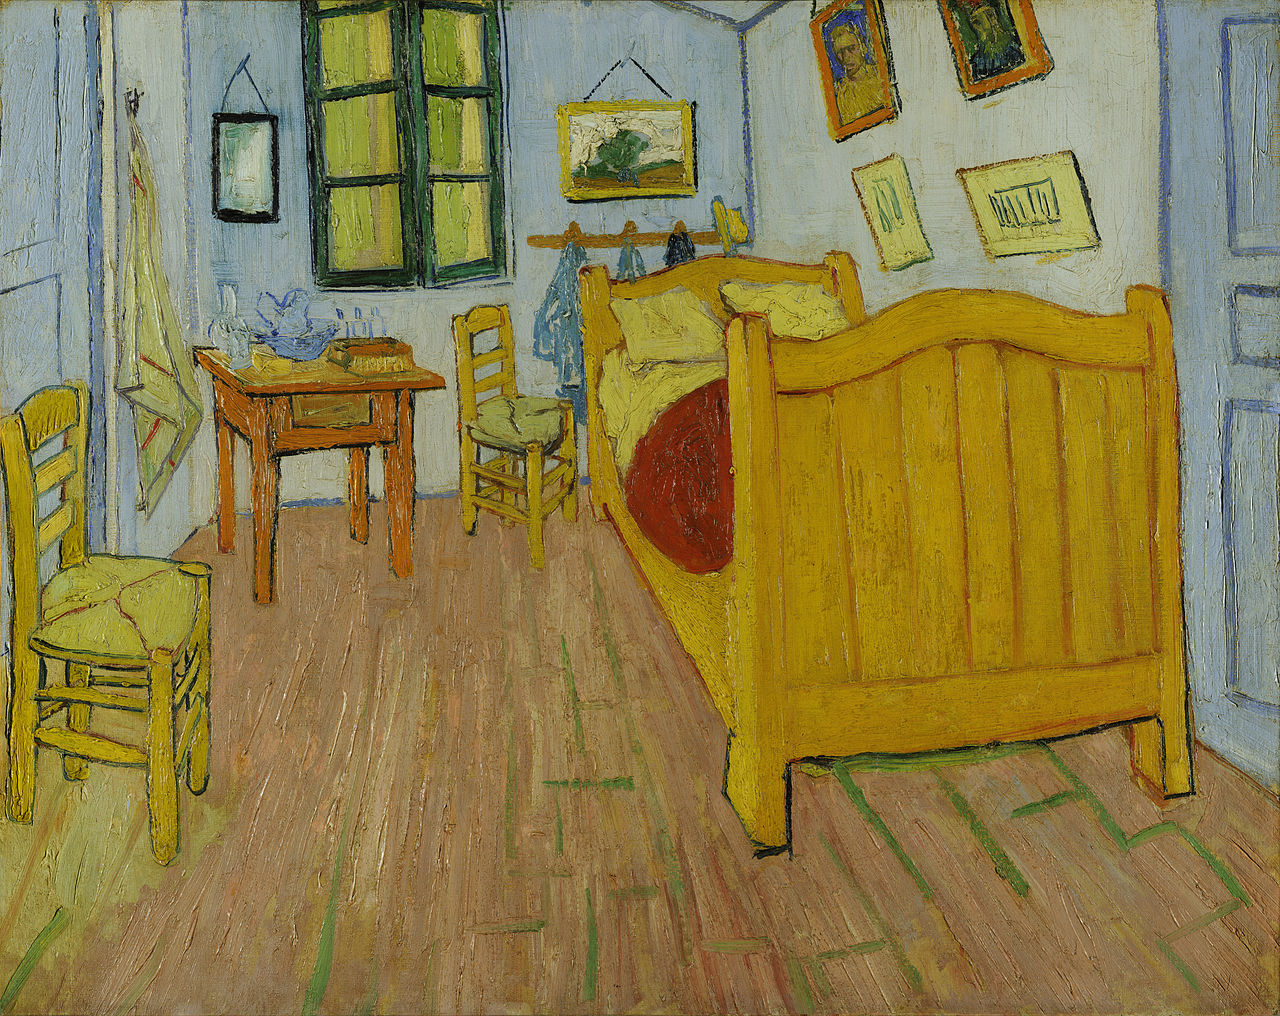
\includegraphics[height=0.6\textheight,keepaspectratio] {slaapkamer.jpg}
  \caption{Quarto de Van Gogh em Arles}
\end{figure}

Não sabemos se Van Gogh conheceu de Maistre, mas talvez possamos dizer
que, fechado nesse quarto por doença (\cite{goghroom}), terá concebido
estes quadros em condições muito semelhantes às do escritor - e também
razoalvemente inquieto - pelo menos a julgar por uma carta que remeteu
ao seu irmão Theo, onde tenta descrever a composição: ``Enfim la vue
du tableu doit reposer la tête''. Ao reler a carta acrescenta de um
modo igualmente enigmático e em letra mais pequena ``ou plutôt la
imagination'' (Van Gogh 1988).

\subsection{Do outeiro ao acidente}

Em última instância, o tema da ``Viagem à volta do meu quarto'' é a
construção do próprio livro. Apesar das promessas do escritor,
defrauda-se logo o leitor incauto que esperasse o mínimo de
estabilidade estrutural feita da coincidência entre os 42 dias de
cárcere e os 42 capítulos, como se de uma viagem minimamente normal se
pudesse vir a tratar, em que se percorresse o espaço físico do quarto
com lentidão ou minúcia absurdas.

Pelo contrário, a única que subsiste da analogia capítulo-dia é a
disparidade entre todos eles. As agitações metafísicas ou sentimentais
do protagonista ecoam-se na forma do livro: como dias, há capítulos
puramente indolentes e outros enérgicos e resolutos. Há capítulos
muito curtos onde nada mais se faz do que esperar pelo próximo ou se
evoca o capítulos passados.

Cada capítulo do livro é um esboço inacabado que da sua própria vida
curta, abandonada displicentemente em desastre, como um Desenho, dos
quais restam uns escombros de ideia. E cada capítulo é um atentado
contra todos os outros.

O capítulo XII da ``Viagem...'' é sem dúvida o mais insólito. Ei-lo,
integralmente:

\begin{verbatim}
  . . . . . . . . . . . . . . .
  . . . . . . . . . . . . . . .
  . . . . . o outeiro . . . . .
  . . . . . . . . . . . . . . .
  . . . . . . . . . . . . . . .
  . . . . . . . . . . . . . . .
\end{verbatim}

``O outeiro'' de que fala de Maistre é o local que recordou, no
capítulo anterior em que limpava o pó a um retrato, de ver pela última
vez um amor predilecto.

A emoção é tão forte, que esse outeiro acaba por eclipsar todos os
outros ``pensamentos desconexos'' um capítulo inteiro (``os meus
esforços são baldados [...] é uma etapa militar''). (de Maistre, p???)

De Maistre transforma o outeiro, pequena elevação de terreno,
possivelmente o mais modesto dos acidentes geográficos, numa fonte de
ausência e de assombro. Não só convida o leitor a imaginá-lo como
quase o obriga, enquanto dele se diz nada. Enquanto outros seus
contemporâneos românticos escreverão sobre montanhas nevadas ou
planícies verdejantes, de Maistre abriga tudo num outeiro, ou seja em
nada. E este paradoxo, perfeitamente consistente com o da viagem
imóvel, é talvez ainda mais poderoso que ele.

Martin Heidegger, que por coincidência também escrevia em retiro,
concebe uma ideia semelhante n'``A Origem da Obra de Arte'', e
precisamente acerca de uns sapatos de camponês pintados pelo pintor de
quartos que apontámos no capítulo anterior (\cite[p.24]{heidegger}):

\begin{quote}
  A partir da pintura de Van Gogh não podemos sequer estabelecer onde
  se encontram estes sapatos.[...] Um par se sapatos de camponês e
  nada mais. E todavia...  Na escura abertura do interior gasto dos
  sapatos, fita-nos a dificuldade e o cansaço dos passos do
  trabalhador.
\end{quote} 

REVER: Ou seja o nada do outeiro, como abertura escura, não só existe como
nos fita e nos interpela.

Na poesia, o ``nada'' é curiosa predilecção de algum poetas de língua
portuguesa do século XX, como Fernando Pessoa ou Manoel de Barros
\cite{manoel}:

\begin{quote}
  ``Há tanta suavidade em nada se dizer / E tudo se entender — ''
\end{quote}
Fernando Pessoa \cite{pessoa}


\begin{quote}
``Há muitas maneiras sérias de não dizer nada, mas só a poesia é verdadeira''
\end{quote}
Manoel de Barros \cite{manoelverso}

O poeta brasileiro tem também um poema n``O livro das ignorâças''
propósito de uma enseada, que se pode ouvir \emph{on-line} dito pelo
próprio autor em \cite{avidaebreve}.

\begin{quote}
  O rio que fazia uma volta atrás de nossa casa
era a imagem de um vidro mole que fazia uma
volta atrás de casa.
Passou um homem depois e disse: Essa volta
que o rio faz por trás de sua casa se chama
enseada.
Não era mais a imagem de uma cobra de vidro
que fazia uma volta atrás de casa.
Era uma enseada.

Acho que o nome empobreceu a imagem. 
\end{quote}

Ainda que aqui seja, inversamente a de Maistre, o nome que devora a
imagem, este poema encontra-se muito próximo do lugar poético que o
``outeiro'': afirma a elipse como figura de estilo e a ausência como
fonte imagética.

Nos dois casos, a ideia de \emph{acidente geográfico} não parece ser
casual; um \emph{acidente} não é um acontecimento qualquer. No limite
não pode ser descrito - da mesma forma que, ainda que de Maistre o
tenha tentado quando examinava velha correspondência, não conseguiu
descrever um traço ou uma pincelada sem se
emocionar. \cite[p.xxx?]{demaistre}

A palavra ``acidente'' abunda na pequena viagem. (\cite[pxxx, pxxx,
  pxxx, pxxx, pxxx]{demaistre}) Por fim, é o próprio de Maistre que,
na ``Expedição nocturna...''  sente a necessidade consagrar um
capítulo à sua estratégia compositiva acidental
(\cite[p.xxx?]{demaistre}):

\begin{quote}
  Tinha uma velha parente, mulher de muita inteligência, cuja conversa
  era das mais interessantes; a sua memória, porém, inconstante e
  fértil a um tempo, fazia-a passar muitas vezes de um episódio a
  outro e de uma divigação a outra, a ponto de ver-se obrigada a
  implorar a ajuda de quem a ouvia: ``Que é que vos queria contar?'',
  dizia ela, e muitas vezes também os seus ouvintes se tinham
  esquecido, o que deixava toda a gente num apuro difícil de
  expressar. Ora, pôde notar-se que o mesmo acidente se verifica
  frequentemente nas minhas narrações, e devo convir, efectivamente,
  que o plano e a ordem da minha viagem são exactamente decalcados da
  ordem e do plano das conversas da minha tia; mas não peço o auxílio
  de ninguém, pois reparei que o assunto volta por si mesmo e no
  momento que menos espero.
\end{quote}

\section{Conclusão}

Com este texto espero ter demonstrado que à viagem imóvel, à paródia
lúdica, à política e ao exílio sentimental, que a todos estes estratos
que se econtram na ``Viagem à volta do meu quarto'' se pode somar
outro de natureza puramente estética: o livro é uma espécie de manual
de composição, um manual de espeleologia da própria imaginação, do
qual se retiram consequências para a criação plástica em qualquer das
suas linguagem, mas talvez mais para o desenho e a pintura, tanto mais
que o a indepedência do tema é afirmada repetidamente pelo paradoxos e
acientes.

Mas, se nas viagens que fizemos por ele o quarto de Maistre nos fitou
com este aspecto de manual de pintura ou caderno de desenhos, outras
viagens serão possíveis. Aliás, como se observa no prefácio, as
diferenças entre a ``Viagem...'' e a ``Expedição nocturna...'', mostra
precisamente que uma viagem, como um acidente, é uma coisa
irrepetível.

\printbibliography[heading=bibliography,title={Bibliografia}]

\end{document}

%% Local Variables:
%% coding: utf-8
%% End:
